%% Can you also try and add some paragraphs? You can use the \par command.

CMOS(complementary metal oxide semiconductor) sensors are one of the most commonly used modern methods of creating digital images in cameras.  \autoref{fig:filters} illustrates how light passing from the outside passes through a glass lens and a color filter before finally reaching the photo-diodes.
\begin{figure}[H]
    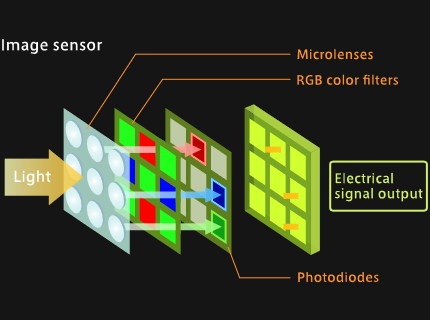
\includegraphics[scale= .5]{assets/ImageSensor.png}
    \caption{CMOS Image Sensor}
    \label{fig:filters}
\end{figure}
The photo-diode is sensitive to light and is able to generate a current by being exposed to photons.  Finally that signal is sent to a central processor and translated into a pixel.(Tokyo Electron Museum)  CMOS sensors are very vulnerable to faults due to radiation and other interference because in some way the circuit has to be exposed to incoming rays and cannot be fully insulated. \autoref{fig:CMOS} shows a basic schematic for a CMOS sensor.  The photo diode has to be exposed to the incoming light so that it can activate the circuit, however, this makes it vulnerable to any other interference that can potentially harm the sensor.  
\begin{figure}[H]
    
\includegraphics[scale= .75]{assets/Cmos schemateic.png}
    \caption{Basic CMOS Active Pixel}
    \label{fig:CMOS}
\end{figure}
One fault that often occurs in CMOS sensors is a Dark Current.  A dark current is when the CMOS circuit is activated by a wave that is not a photon.  In space and other radiation intensive environments this is a very relevant limitation of the technology because extreme accuracy is required with very high consistency.  Radiation that reaches a sensor is likely to cause the sensor to have some kind of fault, and if the intensity of the radiation is high enough then a pixel can become permanently damaged.  These Dark Currents when realized through the circuit and the central processor would appear to be a noisy picture or a collection of white pixels.  These faults can be harmless at first, but given enough time to build up they can render a sensor useless.